% Watbridge Hotels & Suites — Pitch Deck
% Compiles with LuaLaTeX
\documentclass[aspectratio=169]{beamer}
\usepackage{fontspec}
\usepackage{graphicx}
\usepackage{tikz}
\usetikzlibrary{positioning}
\usepackage{pgfplots}
\pgfplotsset{compat=1.16}
\usepackage{xcolor}
\usepackage{hyperref}
\usepackage{array}
\usepackage{tabularx}
\usepackage{multicol}
\usepackage{enumitem}
\setmainfont{Noto Sans}
\definecolor{wbBlue}{HTML}{1F4E79}
\definecolor{wbRed}{HTML}{B22222}
\definecolor{gray9}{HTML}{333333}
\definecolor{gray6}{HTML}{777777}
\hypersetup{colorlinks=true,linkcolor=wbBlue,urlcolor=wbBlue}
\usetheme{Madrid}
\usecolortheme[named=wbBlue]{structure}
\setbeamercolor{title}{fg=white,bg=wbBlue}
\setbeamercolor{frametitle}{fg=wbBlue}
\setbeamercolor{block title}{fg=white,bg=wbBlue}
\setbeamercolor{block body}{bg=gray!5}
\setbeamercolor{itemize item}{fg=wbBlue}
\setbeamercolor{itemize subitem}{fg=wbRed}
\setbeamertemplate{navigation symbols}{}
\setlist[itemize]{topsep=2pt,itemsep=4pt,parsep=0pt,leftmargin=1.4em}

% Title info
\title{Watbridge Hotels \& Suites}
\subtitle{Grow Direct Bookings and Event Revenue in 90 Days}
\author{Capy Digital}
\institute{Uyo • Lagos • San Francisco}
\date{\today}

% Helper: notes box macro
\newcommand{\notes}[1]{\vspace{0.3em}{\footnotesize\color{gray6}\textit{Notes:} #1}}

\begin{document}

% Slide 1 — Title
{\setbeamertemplate{background canvas}{\tikz[remember picture,overlay]{\fill[wbBlue] (current page.south west) rectangle (current page.north east);}}%
\begin{frame}[plain]
  \vspace{0.4cm}
  {\color{white}\LARGE\bfseries Watbridge Hotels \& Suites}\\[4pt]
  {\color{white}\large Grow Direct Bookings and Event Revenue in 90 Days}\\[10pt]
  \tikz{\fill[wbRed] (0,0) rectangle (10,0.15);}\\[6pt]
  {\color{white}\small Uyo, Nigeria}\hfill{\color{white}\small Capy Digital}
\end{frame}}

% Slide 2 — Current state audit
\begin{frame}{Current state audit}
\begin{columns}[T]
\begin{column}{0.6\textwidth}
\begin{itemize}
  \item No HTTPS/SSL; browser warnings reduce trust.
  \item No modern booking engine; no live rates/availability.
  \item Slow, image-heavy pages; poor mobile Core Web Vitals.
  \item Thin SEO; limited schema; under-indexed events and rooms.
  \item Weak CTAs; no WhatsApp click-to-chat; no remarketing/analytics.
\end{itemize}
\end{column}
\begin{column}{0.38\textwidth}
\begin{block}{Screens \& issues}
\vspace{1mm}\centering\fbox{\parbox{0.8\linewidth}{\centering Site screenshots\newline (placeholder)}}\\[2mm]
\scriptsize SSL off • No booking • Slow pages
\end{block}
\end{column}
\end{columns}
\notes{We’ll validate this with a formal audit (Lighthouse, crawl, analytics baseline) in Week 1.}
\end{frame}

% Slide 3 — Business goals & KPIs
\begin{frame}{Business goals \& KPIs}
\begin{multicols}{2}
\begin{itemize}
  \item Direct booking share: +10–25pp vs OTAs
  \item Event/banquet leads: +30–60/mo
  \item Page speed: LCP <2s on 4G
  \item Occupancy lift: +2pp from CRO/SEO
  \item Review rating: 4.5+ with automation
\end{itemize}
\columnbreak
\begin{itemize}
  \item WhatsApp engagement: +20–40/mo
  \item Organic traffic: +40–80\% YoY
  \item Remarketing CTR: 2–4\%
  \item Dashboarding: monthly board-ready report
\end{itemize}
\end{multicols}
\notes{We set a baseline in Week 1 and track weekly in Looker Studio.}
\end{frame}

% Slide 4 — Solution architecture
\begin{frame}{Solution architecture}
\centering
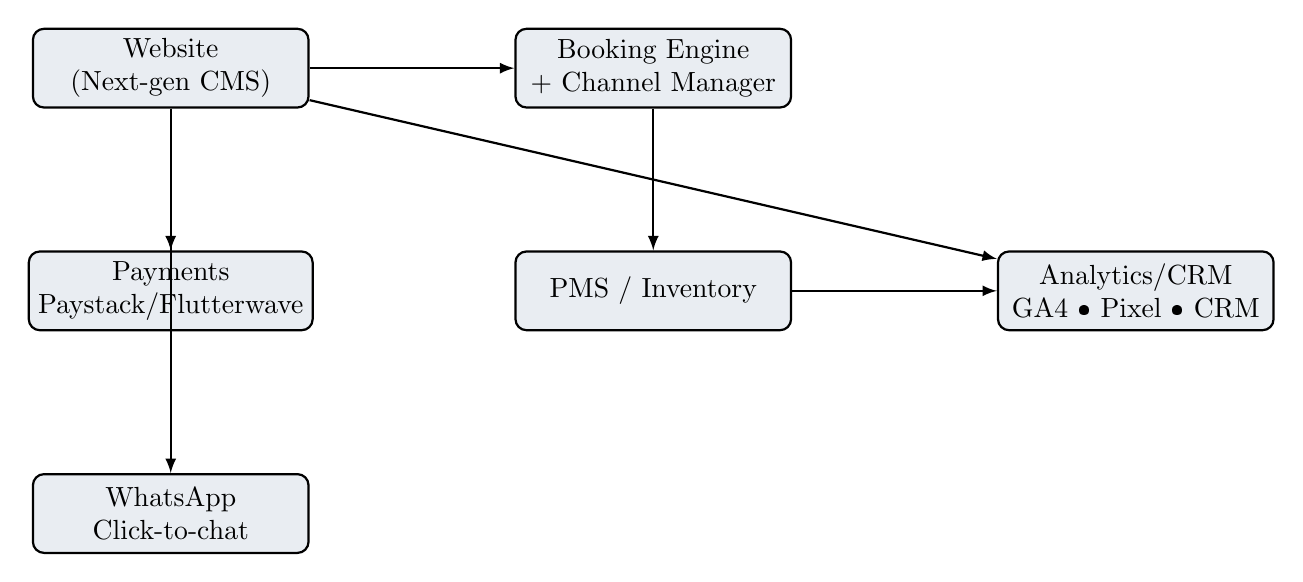
\begin{tikzpicture}[node distance=1.8cm,>=latex]
  \tikzstyle{box}=[draw,rounded corners,thick,align=center,minimum width=3.5cm,minimum height=1.0cm]
  \node[box,fill=wbBlue!10] (site) {Website\\(Next-gen CMS)};
  \node[box,right=2.6cm of site,fill=wbBlue!10] (be) {Booking Engine\\+ Channel Manager};
  \node[box,below=of be,fill=wbBlue!10] (pms) {PMS / Inventory};
  \node[box,below=of site,fill=wbBlue!10] (pay) {Payments\\Paystack/Flutterwave};
  \node[box,below=of pay,fill=wbBlue!10] (wa) {WhatsApp\\Click-to-chat};
  \node[box,right=2.6cm of pms,fill=wbBlue!10] (ana) {Analytics/CRM\\GA4 • Pixel • CRM};
  \draw[->,thick] (site) -- (be);
  \draw[->,thick] (be) -- (pms);
  \draw[->,thick] (site) -- (pay);
  \draw[->,thick] (site) -- (wa);
  \draw[->,thick] (site) -- (ana);
  \draw[->,thick] (pms) -- (ana);
\end{tikzpicture}
\vspace{0.4em}
\notes{Vendor chosen during discovery: HotelRunner/BookOne (value) or Cloudbeds (premium).}
\end{frame}

% Slide 5 — Booking & Payments
\begin{frame}{Booking \& Payments details}
\begin{itemize}
  \item Two clear paths: \textbf{Pay online now} (Paystack/Flutterwave) or \textbf{Reserve now, pay at check-in}.
  \item Support refundable/non-refundable rates, promo codes, and add-ons (breakfast, airport pickup, late checkout).
  \item Card holds/pre-authorizations for no-show protection where applicable.
  \item Front-desk POS flow: map POS posting to PMS folio; nightly reconciliation.
  \item Secure HTTPS, PCI DSS-aligned practices; no card data on website servers.
\end{itemize}
\notes{We keep UX simple: one click to pick payment path; WhatsApp assist available.}
\end{frame}

% Slide 6 — Events & F&B funnels
\begin{frame}{Events \& F\&B funnels}
\begin{itemize}
  \item Banquet/meetings lead forms with required details (date, pax, setup, budget).
  \item Instant WhatsApp routing to sales with SLA and auto-responder.
  \item Dining/poolside pages with menus, promos, and reservation CTA.
  \item Photo/video/360 content to showcase spaces and past events.
  \item CRM handoff with tagging; follow-up templates and reminders.
\end{itemize}
\notes{Goal: shorter lead-to-tour cycle and higher close rate.}
\end{frame}

% Slide 7 — ROI scenarios with chart
\begin{frame}{ROI scenarios — monthly impact}
\small Assumptions: 72 rooms; ADR ₦30,000; OTA commission 15\%; monthly capacity 2,160 nights; 65\% occupancy baseline.
\begin{center}
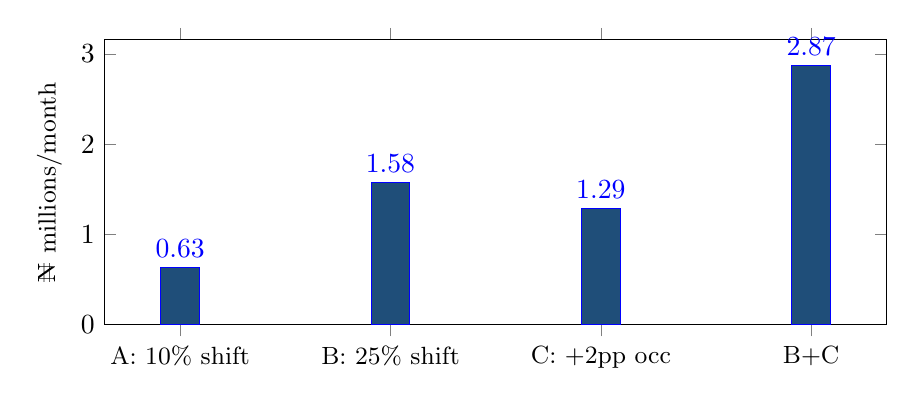
\begin{tikzpicture}
\begin{axis}[
  ybar, ymin=0, width=0.95\linewidth, height=5.2cm,
  ylabel={₦ millions/month},
  symbolic x coords={A: 10\% shift,B: 25\% shift,C: +2pp occ,B+C},
  xtick=data,
  bar width=14pt,
  nodes near coords, nodes near coords align={vertical},
  enlarge x limits=0.12,
  ylabel style={font=\small}, xticklabel style={font=\small,align=center}
]
\addplot+[fill=wbBlue] coordinates {(A: 10\% shift,0.6318) (B: 25\% shift,1.5795) (C: +2pp occ,1.29) (B+C,2.8695)};
\end{axis}
\end{tikzpicture}
\end{center}
\vspace{0.3em}
\begin{tabularx}{\linewidth}{>{\bfseries}l X}
Payback estimate & \raggedright All-inclusive program (₦20,000,000) pays back in ~8–14 months under Scenario B+C allowing for ramp/seasonality. \\
\end{tabularx}
\notes{We will validate baseline OTA mix and occupancy to refine these ranges.}
\end{frame}

% Slide 8 — Pricing & Timeline
\begin{frame}{Pricing \& Timeline}
\begin{columns}[T]
\begin{column}{0.56\textwidth}
\begin{block}{All-inclusive 12-month program — Total ₦20,000,000}
\begin{itemize}
  \item Design/build + booking integration + payments + SEO/perf: ₦8,000,000
  \item PMS/channel manager selection, setup, mapping, training: ₦3,000,000
  \item Content: copywriting + photo/video/360 package: ₦2,000,000
  \item 12-month growth program (SEO/content, CRO, reporting, reputation): ₦5,400,000 (₦450,000/mo)
  \item Contingency/software reserve: ₦1,600,000
\end{itemize}
\end{block}
\begin{block}{Payment milestones}
40\% deposit • 40\% pre-launch • 20\% post go-live
\end{block}
\end{column}
\begin{column}{0.4\textwidth}
\begin{block}{Timeline (10–12 weeks)}
1–2 Discovery\\3–5 Design/Content\\5–7 Build/Integrations\\8–9 UAT/Migration\\10 Launch\\11–12 Stabilization
\end{block}
\end{column}
\end{columns}
\notes{We align dates with your calendar; soft launch mid-week for least risk.}
\end{frame}

% Slide 9 — Proof/guarantee + next steps
\begin{frame}{Proof, guarantee \& next steps}
\begin{itemize}
  \item 90-day conversion guarantee: if direct booking conversion doesn’t improve vs baseline, we provide one month of growth work free.
  \item Deliverables: modern site, booking engine integration, payments, analytics, SEO foundation, staff training, monthly reporting.
  \item Next steps: Approve proposal → Sign MSA → 40\% deposit → Kickoff in 5 business days.
  \item Access needed for discovery: domain/DNS, GA/Pixel, OTA/PMS/channel manager, brand assets.
\end{itemize}
\vspace{0.2cm}
\textbf{Contact} • proposals@capy.ai • +234 (0) 000 0000
\notes{We’ll schedule a joint working session immediately after deposit to align on content and integrations.}
\end{frame}

% Slide 10 — Implementation roadmap (optional)
\begin{frame}{Implementation roadmap by week}
\begin{multicols}{2}
\begin{itemize}
  \item \textbf{W1}: Audit, discovery workshops, KPI baseline
  \item \textbf{W2}: Vendor shortlist (HotelRunner/BookOne/Cloudbeds), contracts
  \item \textbf{W3}: IA, wireframes, content plan, brand polish
  \item \textbf{W4}: Visual design, copy, photo/video shoot
  \item \textbf{W5}: Frontend build, booking engine integration
  \item \textbf{W6}: Payments (Paystack/Flutterwave), WhatsApp, POS mapping
  \item \textbf{W7}: SEO technical setup, schema, performance tuning
  \item \textbf{W8}: GA4/Pixel events, dashboards, UAT
  \item \textbf{W9}: Content migration, bug fixes, training
  \item \textbf{W10}: Launch, monitoring
  \item \textbf{W11}: CRO tweaks, growth program handoff
  \item \textbf{W12}: Board report, roadmap for Q2–Q3
\end{itemize}
\end{multicols}
\notes{We maintain weekly stand-ups and a shared dashboard for transparency.}
\end{frame}

\end{document}
